% no answer key
% \documentclass[letterpaper]{exam}

% answer key
\documentclass[letterpaper, landscape]{exam}
\usepackage{2in1, lscape} 
\printanswers

\usepackage{units} 
\usepackage{xfrac} 
\usepackage[fleqn]{amsmath}
\usepackage{cancel}
\usepackage{float}
\usepackage{mdwlist}
\usepackage{booktabs}
\usepackage{cancel}
\usepackage{polynom}
\usepackage{caption}
\usepackage{fullpage}
\usepackage{comment}
\usepackage{enumerate}
\usepackage{graphicx}
\usepackage{parskip}

\everymath{\displaystyle}


\title{Statistics \\ Homework Five}
\date{\today}
\author{}

\begin{document}

  \maketitle

  \section{Homework}
    \begin{itemize*}
      \item read Chapter 5 
      \item take a look at the ``Check Your Skills'' exercises
      \item exercises: 27-28, 30-34, 37-38, 42, 44-45, 47-48, 51, 53
    \end{itemize*}

  \ifprintanswers
  \else
    \section{Calculations}

    Some of the problems are very tedious to do without a calculator or
    computer that can compute correlation and regression lines.  To make things
    easier, I did some of the calculations on my computer so you'll have the
    numbers even if you don't have a statistics calculator.

    \begin{description}
      \item[34] $r = 0.5581$

        \begin{tabular}{rlrr}
          \toprule
            & variable & mean & sd \\
          \midrule
          1 & Brother & 69.00 & 2.72 \\
          2 & Sister  & 64.00 & 2.57 \\
          \bottomrule
        \end{tabular}

      \item[37]
        \begin{itemize}
          \item with outlier: $r \approx 0.8486$

            \begin{tabular}{rlrr}
              \toprule
                & variable & mean & sd \\
              \midrule
              1 & Neural   & 8.11 & 49.29 \\
              2 & Behave   & 0.66 & 0.51 \\
              \bottomrule
            \end{tabular}

          \item without outlier: $r \approx 0.7015$

            \begin{tabular}{rlrr}
              \toprule
                 & variable & mean  & sd \\
              \midrule
              1  & Neural   & -1.70 & 30.90 \\
              2  & Behave   & 0.57  & 0.39 \\
              \bottomrule
            \end{tabular}

        \end{itemize}

      \item[38]
        All the data sets have about the same numbers:

        $r \approx 0.8164$

        \begin{tabular}{rlrr}
          \toprule
             & variable & mean & sd \\
          \midrule
          1  & x        & 9.00 & 3.32 \\
          2  & y        & 7.50 & 2.03 \\
          \bottomrule
        \end{tabular}

      \item[51] $r \approx 0.9160$

        \begin{tabular}{rlrr}
          \toprule
             & variable & mean  & sd \\
          \midrule
          1  & Stumps   & 2.22  & 1.20 \\
          2  & Larvae   & 25.09 & 15.64 \\
          \bottomrule
        \end{tabular}


      \item[53]
        \begin{itemize}
          \item with 2005: $r \approx 0.5289$

            \begin{tabular}{rlrr}
              \toprule
                & variable & mean  & sd \\
              \midrule
              1 & Forecast & 11.29 & 2.76 \\
              2 & Observed & 12.00 & 4.71 \\
              \bottomrule
            \end{tabular}


          \item without 2005: $r \approx 0.4754$

          \begin{tabular}{rlrr}
            \toprule
              & variable & mean  & sd \\
            \midrule
            1 & Forecast & 11.13 & 2.70 \\ 
            2 & Observed & 11.35 & 3.54 \\ 
            \bottomrule
          \end{tabular}
        \end{itemize}

    \end{description}
  \fi

  \ifprintanswers
    \begin{description}

      \item[27]     
        \begin{figure}[H]
          \centering
          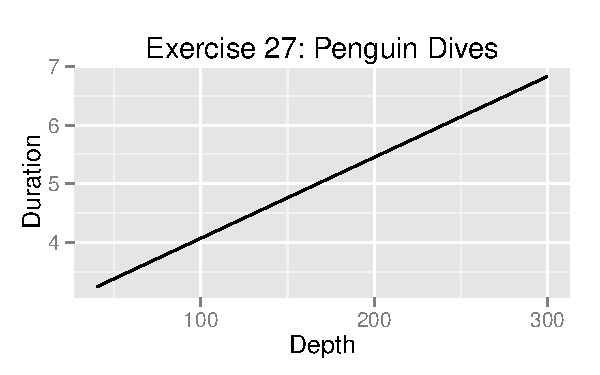
\includegraphics{figures/ex27.pdf}
          \caption{Exercise 27}
        \end{figure}

        \begin{parts}
          \part $m = \unit[0.0138]{m/s}$  Every 0.0138 meters of dive depth takes the
          penguin another second of dive time.

        \part 
          \[
            DD(200) = 2.69 + 0.0138 \cdot 200 \approx \unit[5.45]{s}
          \]
        \end{parts}
    
      \item[28]
        \begin{parts}
          \part for every $\unit[1.507]{mg/l}$ increase in the concentration of TOC,
            there is a $\unit[1]{mg/l}$ increase in the concentration of BOD.

          \part The predicted value is $\unit[-55.43]{mg/l}$.  Perhaps nothing can
            live when the total organic carbon is close to zero, so the BOD value
            doesn't make sense.
        \end{parts}

      \item[30]
        \begin{parts}
          \part 
            \begin{align*}
              y &= 157.68 - 2.993 x \\
              y(30) &= 67.88 \% \\
            \end{align*}

          \part From Figure 5.11, $r^2 = 63.1 \%$
            
          \part Since the correlation coefficient doesn't depend on the order,
          it would be the same magnitude and sign.  The line slopes down, so the
          correlation coefficient is negative:
          \[
            r = - \sqrt{67.88} = -8.24
          \]

        \end{parts}

      \item[31]
        \begin{parts}
          \begin{align*}
            b  & = 0.5 \cdot \frac{2.8}{2.7} \\
               & = 0.5185
            \\
            a  & = 69 - 0.5185 \cdot 64 \\
               & = 35.82 \\
          \end{align*}

          The equation is:
          \[
            \hat{y} = 35.82 + 0.5185 \hat{x}
          \]

          \part
            \begin{figure}[H]
              \centering
              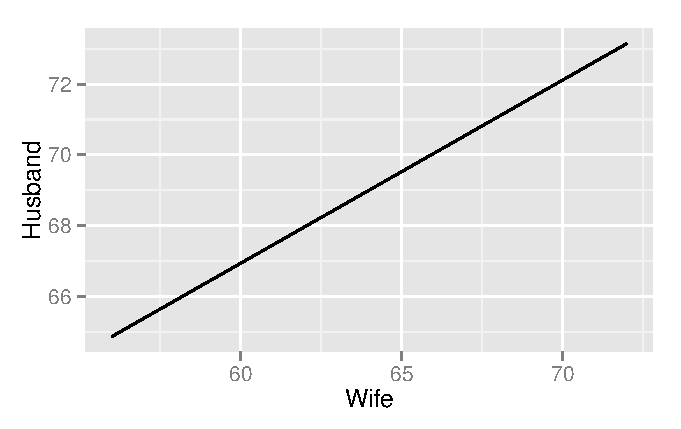
\includegraphics{figures/ex31.pdf}
              \caption{Exercise 31}
            \end{figure}

          \part The estimate isn't very accurate:
            \[
              r^2 = 0.5^2 = 0.25
            \]

            The height relationship only accounts for about 25\% of the variation
            in the heights.
            
        \end{parts}

      \item[32]
        \begin{parts}
          \part
            \begin{align*}
              a & = 0.6 \cdot \frac{75}{280} \\
                & = 0.1607 \\
            \end{align*}

            \begin{align*}
              75 & = 0.1607 \cdot 280 + b \\
              b  & = 30.04 \\
            \end{align*} 

            The equation is:
            \[
              \hat{y} = 30.04 + 0.1607 x
            \]

          \part 
            \[
              y(300) = 78.25
            \]

          \part
            $r^2 = 0.36$.  The earlier scores only account for 36\% of the
            variation in the final score. 
        \end{parts}

      \item[33]
        \begin{align*}
          r^2 & = 0.16 \\
          r   & = 0.4 \\
        \end{align*}

        $r$ is positive because the more classes you attend, the better your
        grade.

      \item[34]
        \begin{parts}
          \part 
            $y = 0.527x + 27.635$
            \begin{figure}[H]
              \centering
              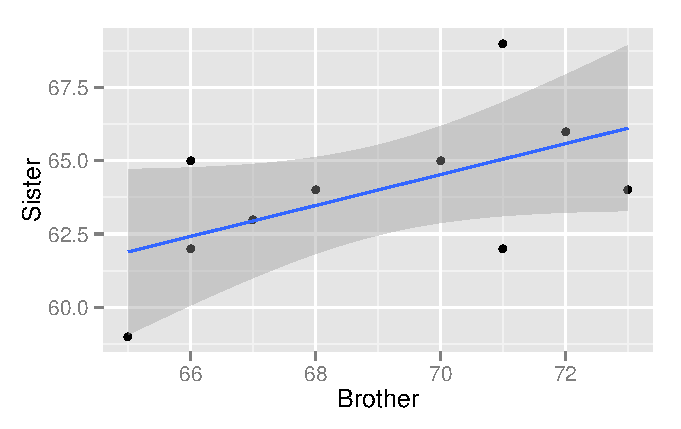
\includegraphics{figures/ex34.pdf}
              \caption{Exercise 34}
            \end{figure}

          \part
            According to the model, Tonya will be about 65 inches tall.  Since
            $r^2$ is only 0.3114, the model only explains 31\% of the variation
            so the prediction probably won't be very accurate.
        \end{parts}

      \item[37]
        \begin{description}
          \item[a-b]
            \begin{figure}[H]
              \centering
              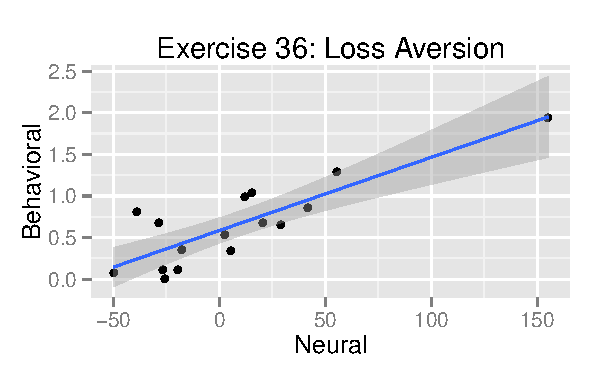
\includegraphics{figures/ex37.pdf}
              \caption{Exercise 37}
            \end{figure}

          \item[c]
            The outlier increases the correlation because it adds a term
            with a high value in both the x and y dimensions.  The outlier
            doesn't affect the regression line much because it is exactly on the
            regression line.

          \item[d]
            \begin{tabular}[H]{lrr}
              \toprule
                        & With Outlier & Without Outlier \\
              \midrule
              slope     & 0.0088       & 0.0089 \\
              intercept & 0.5850       & 0.5858 \\
              $r$       & 0.8486       & 0.7015 \\
              \bottomrule
            \end{tabular}
        \end{description}

      \item[38]
        \begin{figure}[H]
          \centering
          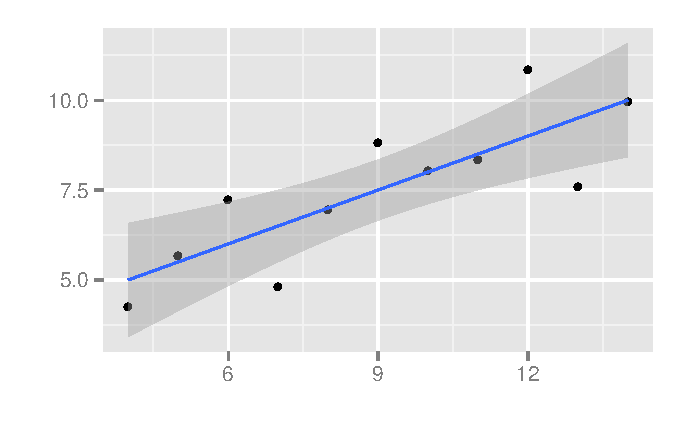
\includegraphics{figures/ex38a.pdf}
          \caption{Exercise 38 (a)}
        \end{figure}

        \begin{figure}[H]
          \centering
          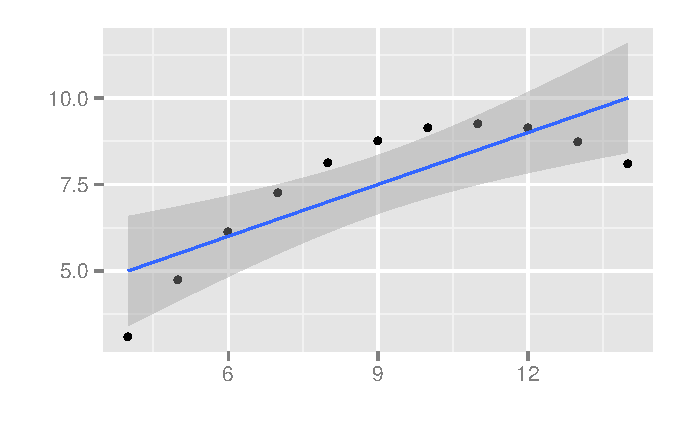
\includegraphics{figures/ex38b.pdf}
          \caption{Exercise 38 (b)}
        \end{figure}

        \begin{figure}[H]
          \centering
          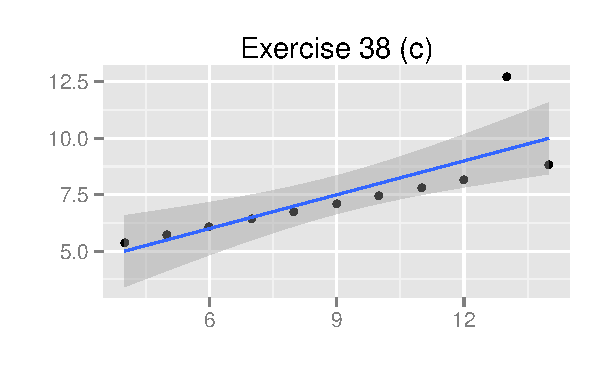
\includegraphics{figures/ex38c.pdf}
          \caption{Exercise 38 (c)}
        \end{figure}

        \begin{figure}[H]
          \centering
          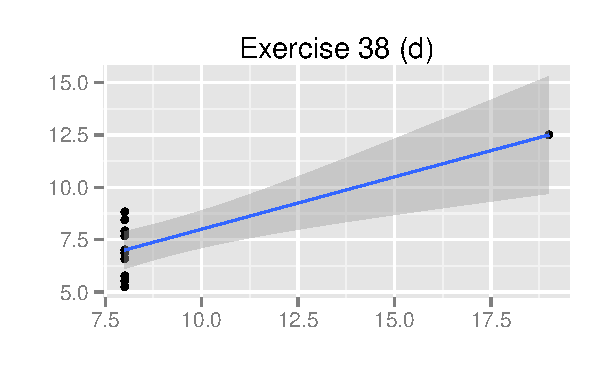
\includegraphics{figures/ex38d.pdf}
          \caption{Exercise 38 (d)}
        \end{figure}

        \begin{description}
          \item[a]
            All of the data sets are about the same.
            \begin{align*}
              y & = 0.5 x + 3 \\
              r & \approx 0.816 \\
            \end{align*}

          \item[c]
            \begin{itemize*}
              \item Graph a looks like a linear relationship, with some minor
                variations.

              \item Graphs b and d don't look like linear relationships.

              \item Graph c looks like a linear relationship with one outlier.
                I would discard the outlier and compute a new regression line.
                It looks like the outlier is drawing the line away from
                where it should be.
            \end{itemize*}
      \end{description}

      \item[42]
        People use artificial sweeteners because they are already overweight.
        Weight is probably causing the sweetener use rather than the other way
        around.

      \item[44]
        Some of the people that previously got B's are now getting A's since A's
        are easier to get.  The SAT hasn't changed, however, so this same group
        of people is still not doing as well on the SAT, bringing the overall
        average for the A group down.

        The same reasoning applies to the other grades.

      \item[45]
        As people get older, they tend to make more money, up to the point when
        they retire.  Consequently, if there are more older but not retired
        people in the workforce, the mean income for the entire workforce goes
        up.

        This argument still applies, even if the median income for older people
        is decreasing over time, as long as it doesn't decrease so much that
        older people no longer make more than younger people.

      \item[47]
        \begin{tabular}[H]{rr}
          \toprule
          First Round & Second Round \\
          \midrule
          70          & 74.53 \\
          80          & 76.33 \\
          \bottomrule
        \end{tabular}

      \item[48]
        Since the regression line passes through $(\bar{x}, \bar{y})$:
        \begin{align*}
          \bar{y} & = 46.6 + 0.41 \bar{x} \\
          \bar{x} & = \frac{\bar{y} - 46.6}{0.41} \\
        \end{align*}

        Antonio's predicted score on the final is:
        \begin{align*}
          \hat{y} & = 46.6 + 0.41 (\bar{x} + 10) \\
                  & = 50.7 + 0.41 \bar{x} \\
        \end{align*}

        We can plug the first equation into the second one to find Antonio's
        final score relative to the final mean:

        \begin{align*}
          \hat{y} & = 50.7 + 0.41 \bar{x} \\
                  & = 50.7 + 0.41 \left( \frac{\bar{y} - 46.6}{0.41} \right) \\
                  & = \bar{y} + 4.1 \\
        \end{align*}

        He should expect to be 4.1 points over the mean on the final.

      \item[51]
        Since $r^2 = 8391$, the stumps account for about 84\% of the variation
        in the larvae.  We can conclude that the beavers are helping the beetles
        by creating the stumps.

        The regression line for larvae based on stumps is:
        \[
          \hat{y} = 11.8937 x - 1.2861 
        \]

        \begin{figure}[H]
          \centering
          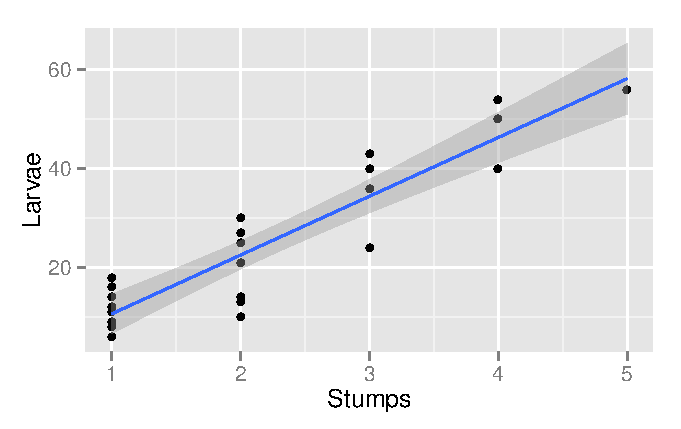
\includegraphics{figures/ex51.pdf}
          \caption{Exercise 51}
        \end{figure}

      \item[53]
        With all the data, $r^2 = 0.2798$.  The prediction accounts for about
        28\% of the variation.  
        
        If you throw out 2005, when he correctly predicted a very bad year, 
        $r^2 = 0.2260$ or only 23\%.

        Either way, the prediction isn't great.

        Including 2005, the regression equation is:
        \[
          \hat{y} = 0.9031 x + 1.8028
        \]

        For a year when he predicts 16 hurricanes, you should actually expect
        around 14 hurricanes.

        \begin{figure}[H]
          \centering
          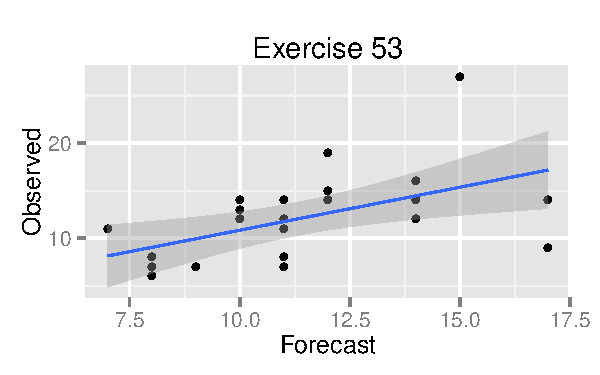
\includegraphics{figures/ex53.pdf}
          \caption{Exercise 53}
        \end{figure}

        \begin{figure}[H]
          \centering
          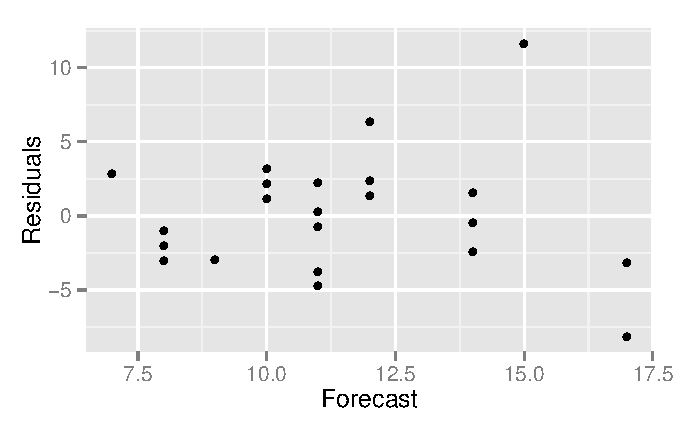
\includegraphics{figures/ex53_residuals.pdf}
          \caption{Exercise 53 Residuals}
        \end{figure}

    \end{description}

  \else
    \vspace{12 cm}
    \begin{quote}
      \begin{em}
        Value judgments are destructive to our proper business, which is
        curiosity and awareness. 
      \end{em}
    \end{quote}
    \hspace{1 cm} --John Cage
  \fi

\end{document}

